\documentclass{standalone}


\usepackage{graphicx}
\usepackage{tikz}

\begin{document}

\begin{tikzpicture}


    \node at (0,0) (i1) {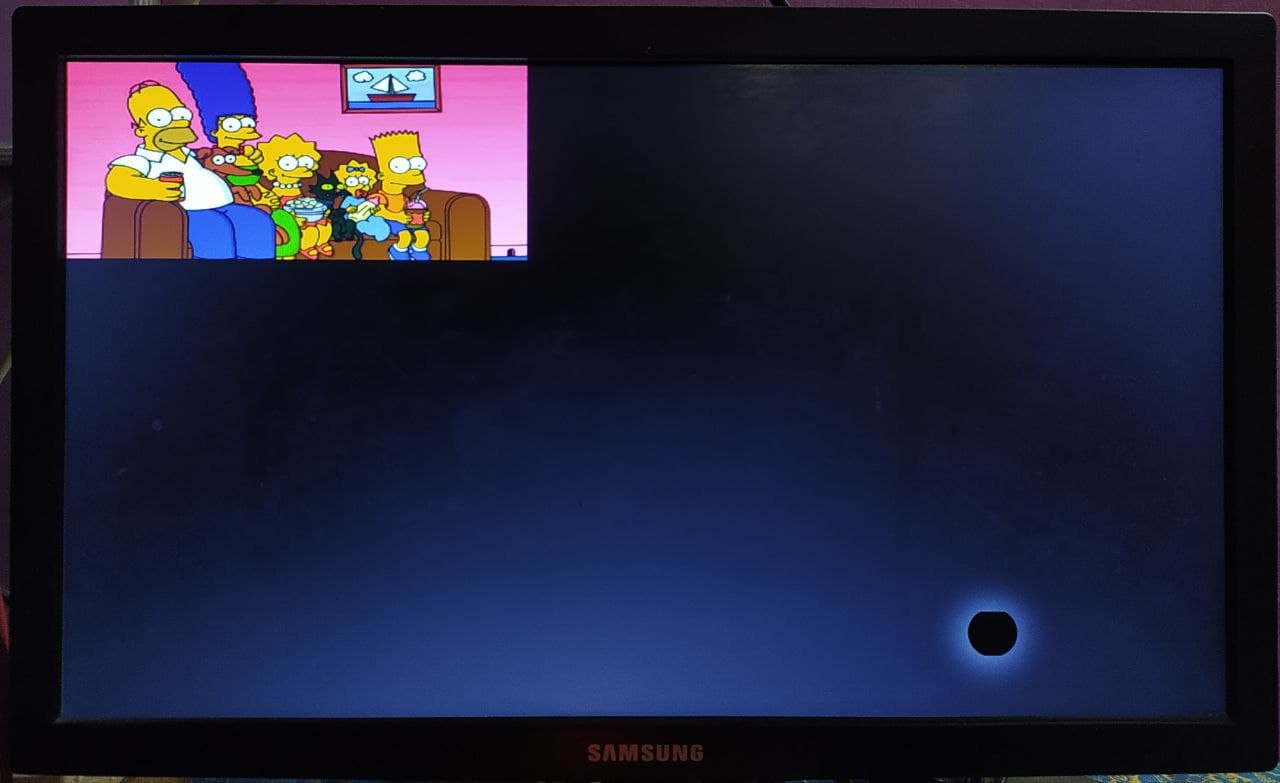
\includegraphics[scale=0.5]{../Outputs/BasicOp_00.jpg}};
    \node at ([xshift=650pt]i1) (i2) {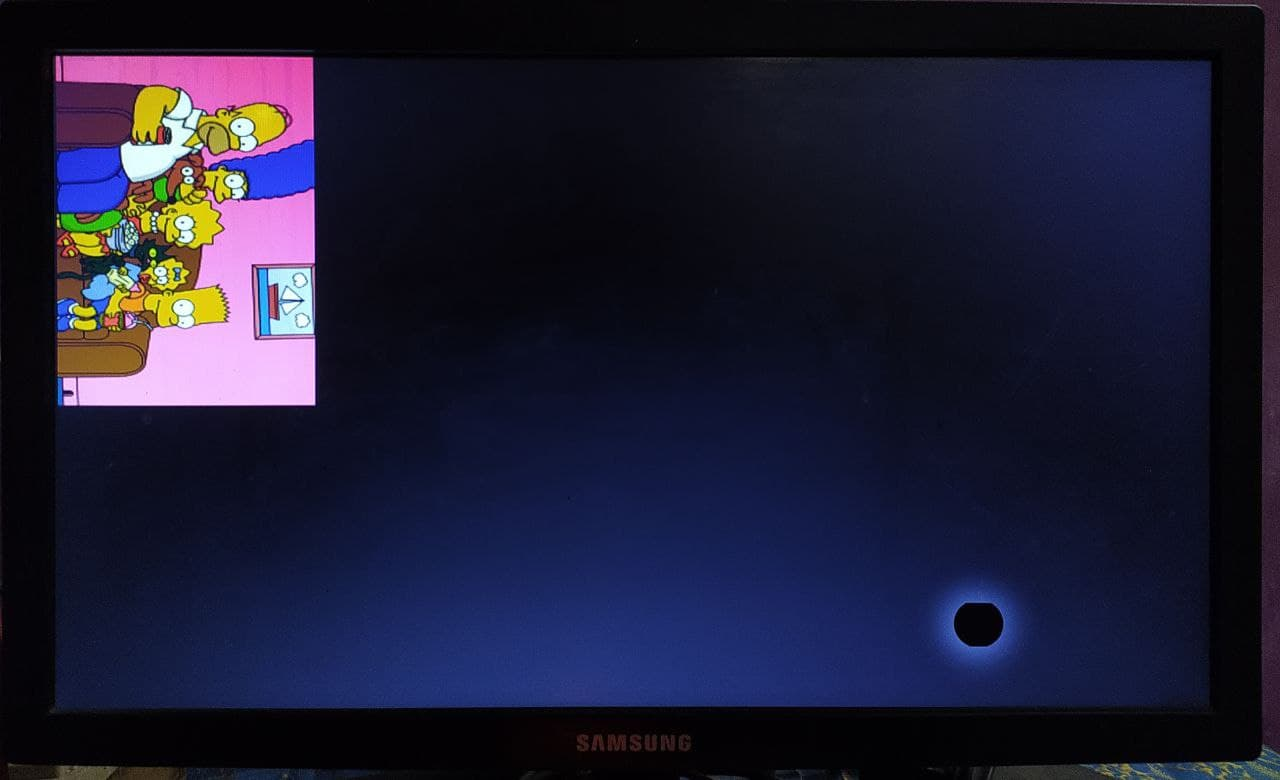
\includegraphics[scale=0.5]{../Outputs/BasicOp_01.jpg}};

    \node at ([yshift=-500pt,xshift=0pt]i1) (i3) {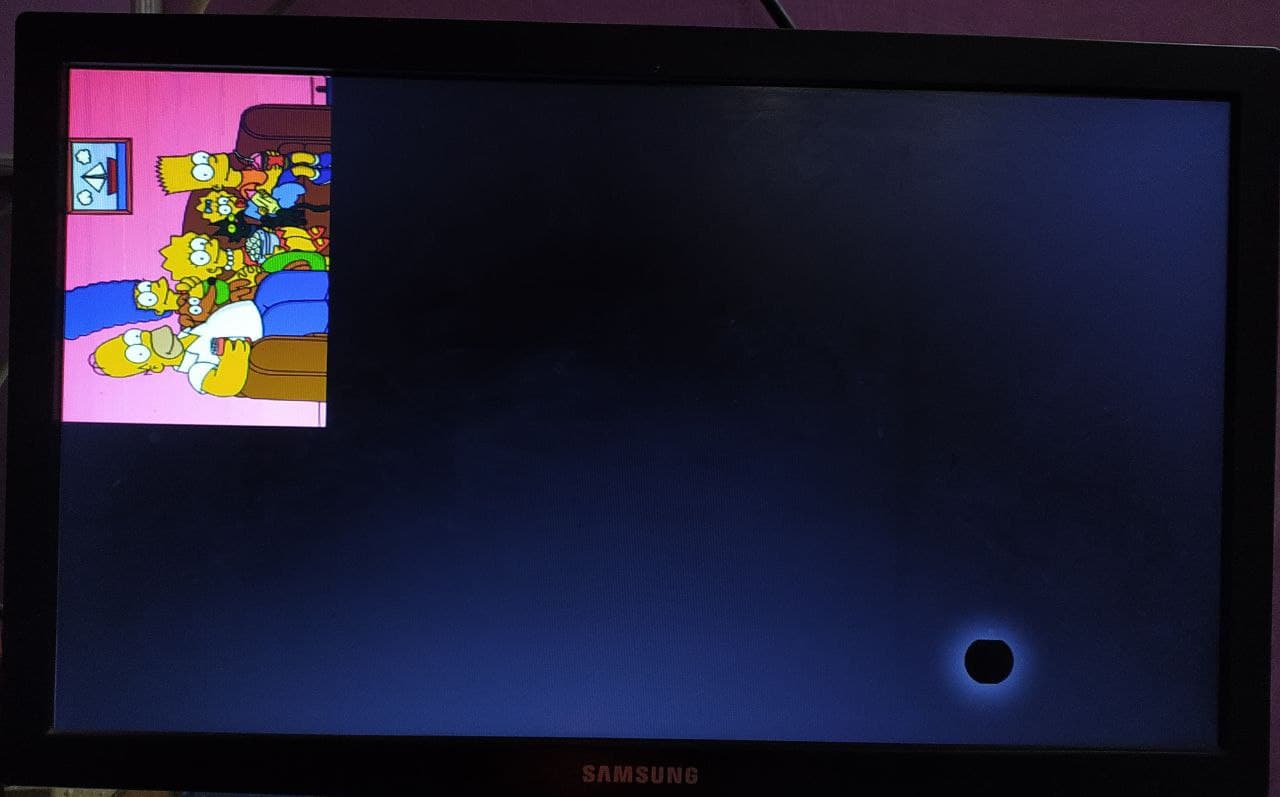
\includegraphics[scale=0.5]{../Outputs/BasicOp_10.jpg}};
    \node at ([yshift=-500pt,xshift=650pt]i1) (i4) {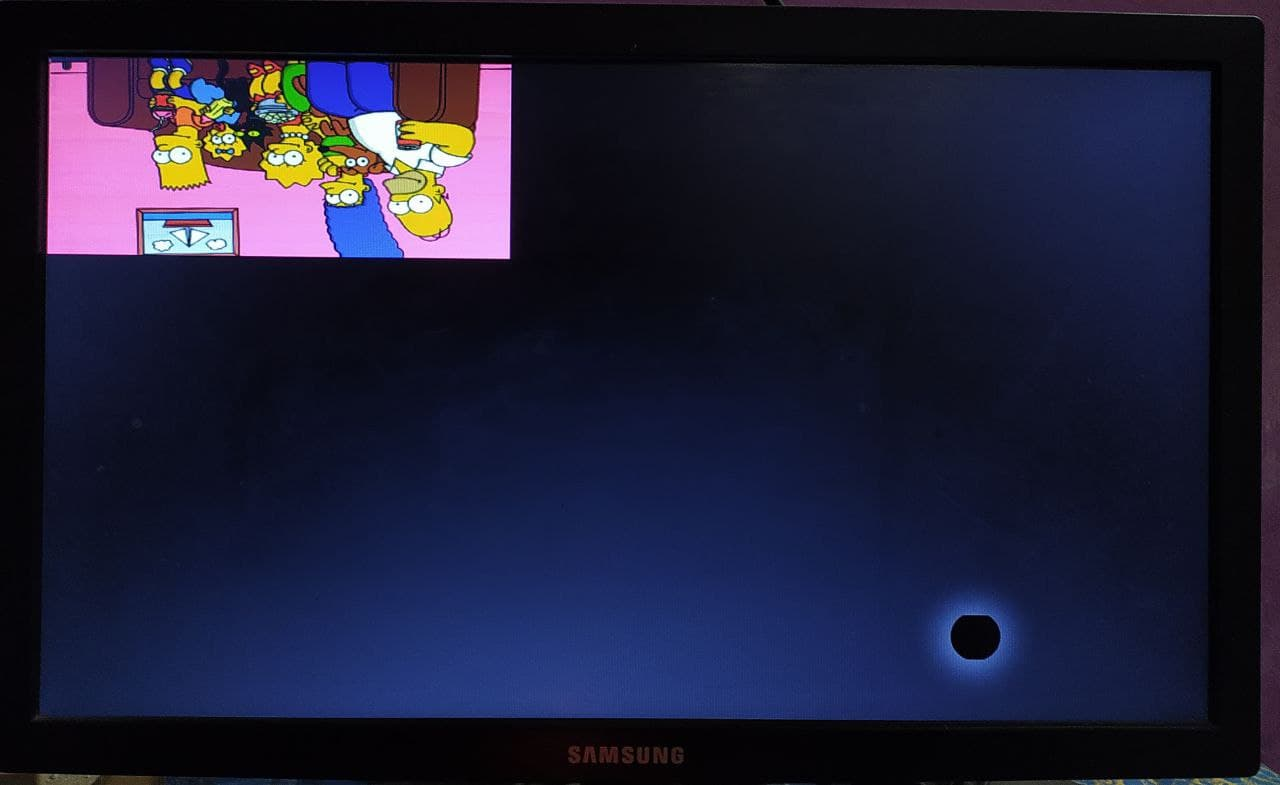
\includegraphics[scale=0.5]{../Outputs/BasicOp_11.jpg}};

    \node at ([yshift=-1000pt,xshift=0pt]i1) (i5) {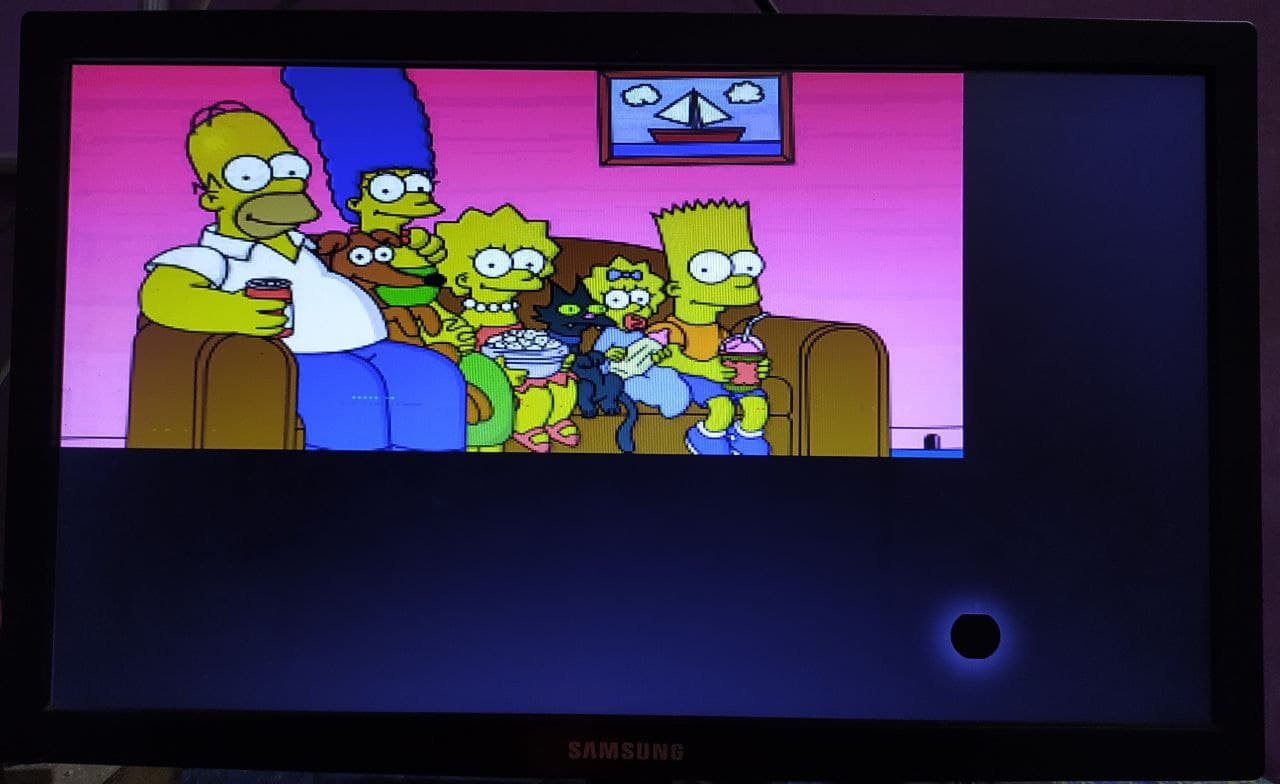
\includegraphics[scale=0.5]{../Outputs/BasicOp_ScaleLARGE.jpg}};
    \node at ([yshift=-1000pt,xshift=650pt]i1) (i6) {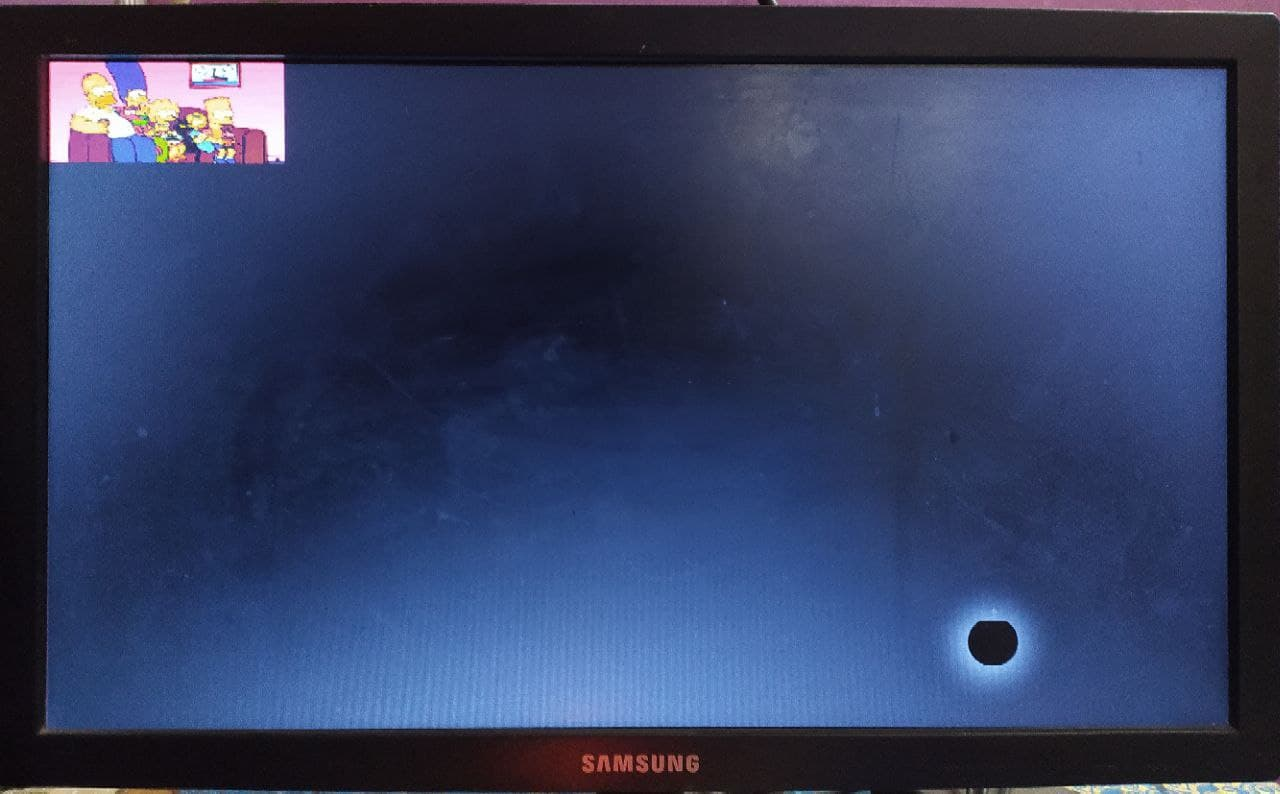
\includegraphics[scale=0.5]{../Outputs/BasicOp_ScaleSMALL.jpg}};


    \node at ([yshift=230pt]i1) {\Huge \textbf{Rotation - rot\_sw == 00}};
    \node at ([yshift=230pt]i2) {\Huge \textbf{Rotation - rot\_sw == 01}};
    \node at ([yshift=230pt]i3) {\Huge \textbf{Rotation - rot\_sw == 10}};
    \node at ([yshift=230pt]i4) {\Huge \textbf{Rotation - rot\_sw == 11}};

    \node at ([yshift=230pt]i5) {\Huge \textbf{Scaling - scala\_sw == 01}};
    \node at ([yshift=230pt]i6) {\Huge \textbf{Scaling - scala\_sw == 10}};

\end{tikzpicture}


\end{document}
